\label{key}\documentclass[bachinf, english ,zihtitle,final,hyperref,utf8]{zihpub}
\usepackage{setspace}
\usepackage{listings}
\usepackage[]{algorithm2e}
\usepackage{floatrow}
\usepackage{subfig}
\setcounter{tocdepth}{1}
\author{Ankur Sharma}
\title{Performance Tuning \& Parallelization of Inchworm Sequence Assembler}
\bibfiles{doku}
\birthday{25. March 1991}
\placeofbirth{Allahabad, India}
\betreuer{Prof. Dr. Wolfgang E. Nagel}
\newcommand*{\captionsource}[2]{%
  \caption[{#1}]{%
    #1%
    \\\hspace{\linewidth}%
    \textbf{Source:} #2%
  }%
}
\begin{document}
\listoffigures
\newpage
\chapter{Introduction} 
RNA-seq is a technology used to study and analyze transcripts. But due to high level of complexity, the reads generated from sequencer are much shorter than the transcripts from which they are derived. As suggested in \cite{trinitynew} and \cite{Trinity}, Trinity software for de novo reconstruction of transcriptomes, provides a novel and efficient way of assembling these short reads together in order to obtain a transcript. This software basically contains three modules namely Inchworm, Chrysalis and Butterfly. Short read sequences, basically represented as a sequence of characters, are piped through these modules one after the other in order to successfully obtain a transcript. The first two modules, Inchworm and Chrysalis are written in C++ whereas the last module Butterfly is written is Java. Based on the significance of this application in present research and development revolving around RNA sequencing, it poses a great challenge to optimize its performance both in terms of time and the results obtained by this application. Based on my analysis, I realized that Inchworm module could be optimized without much alter in the results of Trinity as a whole. So the main target of this work was to achieve a performance boost  without altering the core algorithm and approach of the application. The thesis describes the performance bottlenecks that were discovered during the analysis of the application as well as the measures that resulted in a significant performance boost of Inchworm.
\section{Biological Background}
The detailed analysis of  an assembly tool like \emph{Inchworm} involves familiarity with a lot of biological terms and techniques. This section discusses some of the key biological elements that play crucial role in understanding the biological significance of what is being done and why it is done in this application. Some of the important terms frequently used in this documentation are discussed below:
\subsection{Key Terms}
\paragraph{Deoxyribonucleic Acid (DNA)}: It is a biological molecule that holds the information and instruction that is used for the development and proper functioning of all living organisms. As shown in figure \ref{dna}, it has a double stranded helical structure that are coiled around each other. Both of these strands hold similar information which is replicated when these strands get separated. In general terms, this is an information storage system that holds information and helps in transferring this information genetically from generation to generation of a living cell.

\begin{figure}[h]
\center
\subfloat[]{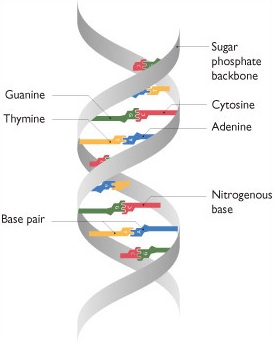
\includegraphics[scale=0.4]{DNA.jpg}\label{dna}}
\hspace{50pt}
\subfloat[]{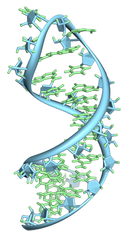
\includegraphics[scale=0.6]{RNA.png}\label{rna}}
\caption{(a) Double stranded DNA, (b) Single stranded RNA molecule}
\floatfoot{Source: \cite{wiki}}
\end{figure}
\paragraph{Ribonucleic Acid (RNA)}: 
This is a biological molecule that helps the living cells in performing roles such as genetic information encoding, decoding, regulation of the genes. It is a single stranded molecule as represented in figure \ref{rna} on page ~\pageref{rna}, and has much shorter chain of nucleotides than DNA molecule. Some of these molecules also play important role within the cells by acting as a catalyst in several biological reactions, controlling gene expressions, or sensing and communicating responses to the cellular signals. 
\paragraph{Nucleotide}: These are organic molecules that serve as a building block of large nucleic acid molecules like DNA and RNA. They carry packets of energy within the cell and plays an important role in metabolism. IUPAC has defined standard symbols for each nucleotide like A (Adenine), G (Guanine), C (Cytosine) and T (Thymine). Most of the other nucleotides like purine and keto can be represented as a combination of these symbols. This is why Trinity deals with assembling sequences containing symbols A, T, G and C.
\paragraph{Reads}: 
Reads are a short sequence of nucleotides which are extracted from transcripts using high-throughput sequencers. These reads can be reassembled together in order to obtain a full length transcript.
\paragraph{K-mer}: It is a k-tuple consisting of characters A,T, G or C that represents the short read sequence. These k-mers are joined together based on the overlapping coverage to obtain a full length transcript.
\paragraph{Sequence Assembly}: Sequence assembly refers to the technique of merging fragments of a longer sequence to reconstruct the original transcript. This is required as sequencing technology cannot report whole genomes in one go, but rather short reads of size between 20 and 30000 bases, depending on which technology is used. Typically the short sequence fragment are called reads.
\paragraph{De Bruijn Graph} A De Bruijn graph of n-dimensions and m-symbols is a directed graph that represents overlapping between different sequences of symbols. A graph with mentioned specification has $m^{2}$ vertices with each symbol appearing multiple times in a sequence and contains all possible sequences of length n of given symbols.
\paragraph{N50 length} For a set of contigs, the N50 length can be defined as the length of contig for which the set of all contigs of this or greater length contains more than half of the total of the lengths of the contigs.
\section{Trinity}
\emph{Trinity} assembler, developed at the Broad Institute, Massachusetts USA and Hebrew University of Jerusalem, represents a method for \emph{de novo} assembly of full-length transcripts that uses construction and analysis of sets of \emph{de Bruijn} graph. It is known as Trinity because it involves three major steps which are integrated together in the form of three different software modules namely Inchworm, Chrysalis and Butterfly. As shown in figure ~\ref{trinity} on page ~\pageref{trinity}, the first stage of Trinity i.e. Inchworm assembles RNA-seq data into linear contigs. It assembles together the k-mers that satisfy certain overlapping criteria like for a k-mer of size k, we join together two k-mers if they overlap in a sequence of length k-1. Then Chrysalis groups contigs which are related due to alternate splicing or gene duplication and constructs de Bruijn graphs. Finally, Butterfly examines reads the contigs of the de Bruijn graph and reports final full length transcripts and isoforms of transcripts.
%%%%%%%%%%%%%%%%%%%%%%%%%%%%
\chapter{Inchworm}
Inchworm first decomposes reads into a catalog of k-mers which is by default 25-mers. It stores the k-mer sequences and the frequency of the k-mers, but not the edges between different k-mers. This allows us to save the memory and the amount of computation that needs to be done on this catalog. The single most abundant k-mer with reasonably good complexity is taken as a seed k-mer. The seed k-mer is then extended on both ends which is guided by the set of overlapping k-mers. For each extension there are four possibilities with k-1 overlap each ending with one of the four possible nucleotides. Each of these k-mers are looked up in the k-mer catalog and its frequency and complexity is determined. The most abundant and complex k-mer is selected from these possibilities and is used for the extension as shown in figure ~\ref{trinity}~(a). This used k-mer is then removed from the catalog to ensure that the k-mer is not reused for any extension. The same procedure continues until the whole k-mer catalog is exhausted. If two possibilities are found to have similar frequency and complexity, Inchworm recursively assembles both the extension following the path of greatest coverage and chooses the k-mer which has the highest amount of cumulative coverage.
\begin{figure}[h]
\center
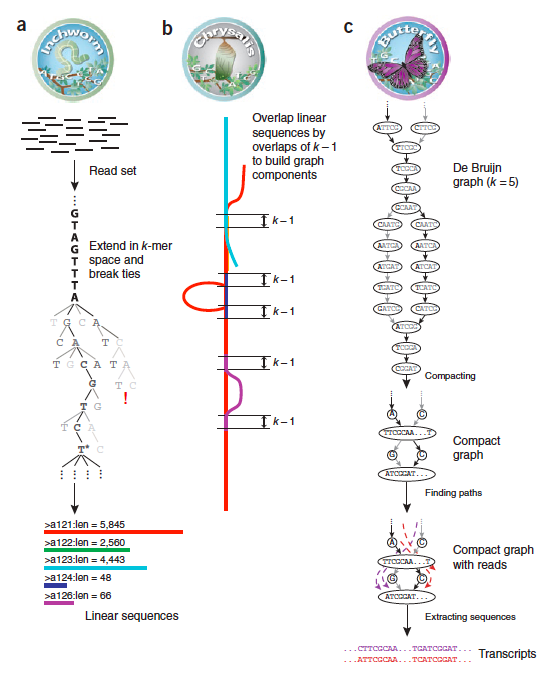
\includegraphics[scale=0.5]{Trinity_phases}
\caption{Trinity - Workflow}
\floatfoot{Source: \cite{Trinity}}
\label{trinity}
\end{figure} 
\section{Phases}
Inchworm can be subdivided into three sub-modules that  are parsing, pruning and assembly through which the data is piped in order to obtain linear contigs. This modular structure enables us to analyze the performance of different sub-modules of Inchworm in an efficient way. It also allows us to optimize each step independently and verify the effects of these optimizations on the final results obtained from Inchworm. In further paragraph, we analyze the working of Inchworm categorized into three sub-modules.  
\subsection{Parsing}
Inchworm uses a catalog of k-mers that holds the k-mer sequence and the frequency of occurence of these k-mers. This catalog is designed using a hash map with the integer equivalent of the k-mer sequence as a key and the frequency of occurrence of that k-mer as the value. FASTA/FASTQ files store reads as shown in figure \ref{fastq}. So, trinity first extracts k-mers  from reads and evaluates the abundance of each k-mer. Initially this step was a part of Inchworm, but  later on the developers used faster k-mer counting tool  \emph{Jellyfish} which is incorporated as an alternative in the Trinity package.
\begin{figure}[h]
\begin{center}
\subfloat[Snippet from fragment file containing reads]{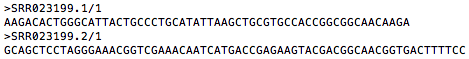
\includegraphics[scale=0.7]{lfa}\label{fastq}}\\
\subfloat[Snippet from file containing extracted k-mer sequences and its abundance]{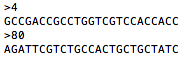
\includegraphics[scale=0.7]{fa}\label{fasta}}
\caption{Snippets from FASTA files}
\end{center}
\end{figure}
\paragraph{} Inchworm reads this k-mer information from the FASTA file and stores it as a key-value pair in the memory in the form of a hash table. These key-value pairs have the integer equivalent of the k-mer sequence as the key and the abundance as the value. These integer equivalent of k-mer sequence is a 2-bit encoded unsigned integer. With the total size of 8-bytes, it can incorporate k-mers upto 32-mers but since 25-mers works very well, the developers leverage 25-mers as a fixed option with Trinity. The integer equivalent of a k-mer sequence is evaluated using simple conversion of each  characters in the sequence and shifting the bits. The following snippet of code from the source evaluates and returns the integer value corresponding to the k-mer sequence.
\begin{center}
\begin{lstlisting}[language=C++]
unsigned long long kmer_to_intval(string kmer) {  
 /* Error checking the kmer for max size*/
  unsigned long long kmer_val = 0;  
  for (unsigned int i = 0; i < kmer.length(); i++) {
	char c = kmer[i];
	// {G => 0 ; A => 1; T => 2 ; C => 3}
	int val = _base_to_int[c];
	// Checking kmer for invalid characters
	kmer_val = kmer_val << 2;
	kmer_val |= val;	
  }  
  return(kmer_val);
}
\end{lstlisting}
\end{center}
\paragraph{} Inchworm can use GNU Hash Map (default), Google's Sparse Hash Map or the  Solaris Studio Hash Map. But since GNU Hash Map has a better performance with respect to access time, it was selected to perform all the final comparisons. The catalog generated by this phase is then used by all the other sub-modules as a database of k-mers throughout the Inchworm run.
\subsection{Sorting}
Once the k-mer catalog is ready, we need to generate a list of k-mers sorted on the basis of decreasing abundance. This is done because the assembly phase can use this list to find the most abundant k-mer which can then be used as a seed k-mer for generating the linear contig. Creating the sorted list of k-mers reduces the time that is required in order to locate the most abundant k-mer from O(N) to O(1), where N is the size of the k-mer catalog.
\paragraph{}
This phase involves basically two steps. In the first step, Inchworm create a copy of all the k-mer sequences using a vector that hold the key-value pair with integer corresponding to k-mer sequence as key and the abundance as the value. It then uses the standard sort algorithm to sort this vector in the decreasing order of the abundance. 
\begin{lstlisting}[language=C++]
\\ #include <algorithm>
sort(kmer_list.begin(), kmer_list.end(), sorter);
\end{lstlisting}
\subsection{Pruning}
The quality of linear contigs obtained from Inchworm highly depends on the complexity of k-mers that are used in the extension of the seed k-mers. The complexity of a k-mer depends on several factors like the abundance, the sequence itself and how well it can be extended. Based on these factors, Inchworm marks the low complex k-mers so that they are not used in the assembly phase. This enhances the complexity and biological significance of the k-mers. This phase of Inchworm uses three different criteria to check the complexity of k-mers : 1. Based on the frequency of the k-mer, which is expected to be above certain threshold; 2. Based on entropy of the k-mer which is evaluated using equation ~[\ref{eq1}], if the entropy is less than certain threshold, the k-mer is removed from the catalog; 3. Based on less complex extension which is evaluated by extending the k-mer for just one forward step, if the ratio evaluated using equation ~[\ref{eq2}] of the frequency of extension k-mer and the dominant frequency for all possible extensions is less than certain fraction (min\_ratio\_non\_error), the seed k-mer and the extension k-mer is removed from the catalog.

\begin{equation}
Entropy = \sum_{x \in \{G,A,T,C\}} \frac{count(x)}{kmer\_length}  * log_2 \bigg(\frac{kmer\_length}{count(x)} \bigg ) 
\label{eq1}
\end{equation}

\begin{equation}
Ratio = \frac{kmer\_count}{dominant\_count}
\label{eq2}
\end{equation}
Since the k-mers with the abundance count equals to zero is not used in the extension, Inchworm removes the k-mers just by setting the count of the k-mers to zero instead of spending time in removing them from the hash table. This approach surely uses a lot of memory which is not freed throughout the execution, but on the other hand, it saves a lot of time which is wasted in removing the k-mers from the hash table and redistribution of space inside hash table.
\begin{figure}[h]
\center
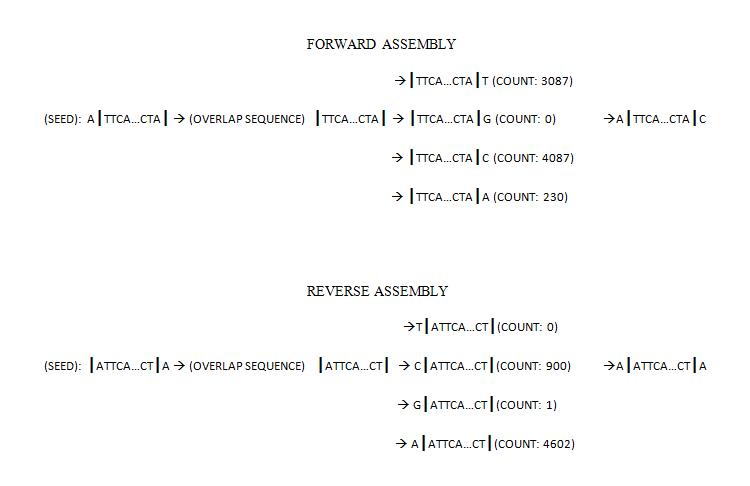
\includegraphics[scale=0.7]{assembly}
\caption{Assembly}
\label{assemble}
\end{figure}
\subsection{Assembly}
Once the sorted list of k-mers is produced, Inchworm uses this list to find the most abundant unused k-mer. This is used as a seed to generate the linear transcript which is obtained by extending the seed in both forward and reverse directions. As shown in figure ~\ref{trinity} on page \pageref{trinity}, Inchworm extends the seed using a simple greedy approach. It creates a dummy extension based on the degree of overlapping which is k-1, extending in all possible ways with nucleotides A,T,G \& C, the assembler then finds the abundance of these dummy extension and selects the best possible option for extension. Similar approach is used in the reverse direction to obtain the reverse extension. Once the seed is extended in both the directions, both of these semi extended transcripts are joined together to obtain the full length linear transcript. Figure \ref{assemble} illustrates how assembly is performed in both forward and reverse direction. Further paragraph discusses the assembly algorithm in a more detailed way.

\paragraph{Algorithm} The assembler picks the k-mers from the sorted list in a top bottom approach which is the most abundant available k-mer. It then checks whether this k-mer has enough count and entropy (equation \ref{eq1}) to be used as seed, and once this verification is complete, the assembler uses this k-mer for extension. Before reporting the full length transcript, the assembler verifies the complexity of this transcript by checking the length of the assembled contig and the average coverage evaluated using equation \ref{eq3}. If the average length is very small or the average coverage is less than the specified limit, the assembly is dropped and a new seed is selected from the sorted list of k-mers. The k-mers used in the extension of the dropped contig are not removed from the catalog. If the linear contig is complex enough to be reported, the assembler marks each of the k-mers that were used in the extension so that they are not used again in further assembly. The seed used in the extension is also marked so that it is never used again as a seed or in any further extensions. For marking the k-mers, assembler either removes the k-mers from the hash table or simply sets the count of the k-mers to 0. Assembler then chooses the next most abundant k-mer as seed and repeats all the steps until whole k-mer catalog is exhausted.
\begin{equation}
Average\ Coverage = \frac{\sum_{} count (k-mer)}{length\ of\ contig} - k-mer\_length
\label{eq3}
\end{equation}

\vspace{20pt}
 \begin{algorithm}[H]
 \KwData{\emph{k}-mer catalog (kcounter)}
 Create sorted k-mer list;\\
 \While{\emph{k}-mer catalog is not exhausted}{
  pick most abundant \emph{k}-mer from the sorted list\;
  \eIf{\emph{k}-mer do not satisfy properties of seed}{
   continue\;
   }{
   evaluate forward assembly\;
   evaluate reverse assembly\;
   create linear-contig by joining forward \& reverse assembly\;
   \eIf{contig is complex enough}{
   	dump the contig to output file\;
   }{
   drop the contig\;
   continue\;
   } 
   }
  }
 \caption{Assembly Algorithm}
\end{algorithm}

%%%%%%%%%%%%%%%%%%%%%%%%%%%%
\chapter{Performance Analysis}
The modular structure of Inchworm eases the process of testing and analysis to a great extent. Each of the parts were analyzed to bring various performance bottlenecks into contrast. The modular analyses allowed a thorough comparison between the original implementation and various counter techniques. Further documentation presents the testing environment specification, various modular analysis techniques adopted for performance analysis, highlights several bottlenecks and optimization techniques that may be used to tackle them. 
\section{Data-sets}
For the performance analysis of Inchworm, I have used \emph{Drosophila melanogaster} and \emph{Schizosaccharomyces pombe} as used by \cite{zhao} and \cite{performance}. More details about these datasets are given in tables 1 and 2.\\
\begin{table}
\begin{center}
\begin{tabular}{| c | c | c | c |}        
\hline            
  Dataset name & \# reads & \# k-mers & \# base pairs \\	\hline
  4M & 1,000,000 & 4,519,455 & 112,986,375 \\  \hline
 39M & 4,066,000 & 39,422,440 & 985,561,000 \\ \hline
 100M & 100,000,000 & 142,308,262 & 3,557,706,550 \\
  \hline  
\end{tabular}
\end{center}
\caption{Dataset details : \emph{Drosophila melanogaster}}
\end{table}
\begin{table}
\begin{center}
\begin{tabular}{| c | c | c | c |}        
\hline            
  Dataset name & \# reads & \# k-mers & \# base pairs \\	\hline
  Schizo & 50,000,000 & 237,578,729 & 5,939,468,225 \\
  \hline  
\end{tabular}
\end{center}
\caption{Dataset details : \emph{Schizosaccharomyces pombe}}
\end{table}
\section{Hardware \& Software Environment}
The performance analysis and measurements of various parameters were conducted on a node of \emph{Taurus} cluster at \emph{Center for Information Services \& High Performance Computing (ZIH), Technische Universit{\"a}t Dresden}, Germany. It consists of three tightly coupled clusters which offers two large shared memory nodes with 1 TB of main memory. The tests were conducted on SMP-Nodes of Taurus which contains two nodes, each with 4x Intel(R) Xeon(R) CPU E5-4650L (8 cores) @ 2.60 GHz and 1 TB of main memory.
\subsection{HPC File Systems}
Taurus currently uses three types of file systems namely SSD (Solid State Disk), scratch and home file system. Sorted on the basis of bandwidth, they offer a great flexibility varying from strong consistency to great speed. SSD is considered as the best option for small I/O operations with the disk size ~50GB. Each taurus node has its own local SSD and multiple processes running on the same node can share the disk. However, the data stored on these disks is ephemeral and is swept automatically after 7 days. Scratch on the other hand is the fastest parallel file system available which offers a high bandwidth. It is shared among all the nodes of the machines. The home file system is a common file system for all HPC machines at ZIH. It is the slowest among the three file systems and smaller than scratch, but offers a great consistency holding multiple backups and the deleted files can be accessed on a logical directory storing the hourly, daily and weekly snapshots.
\begin{figure}[h]
\center
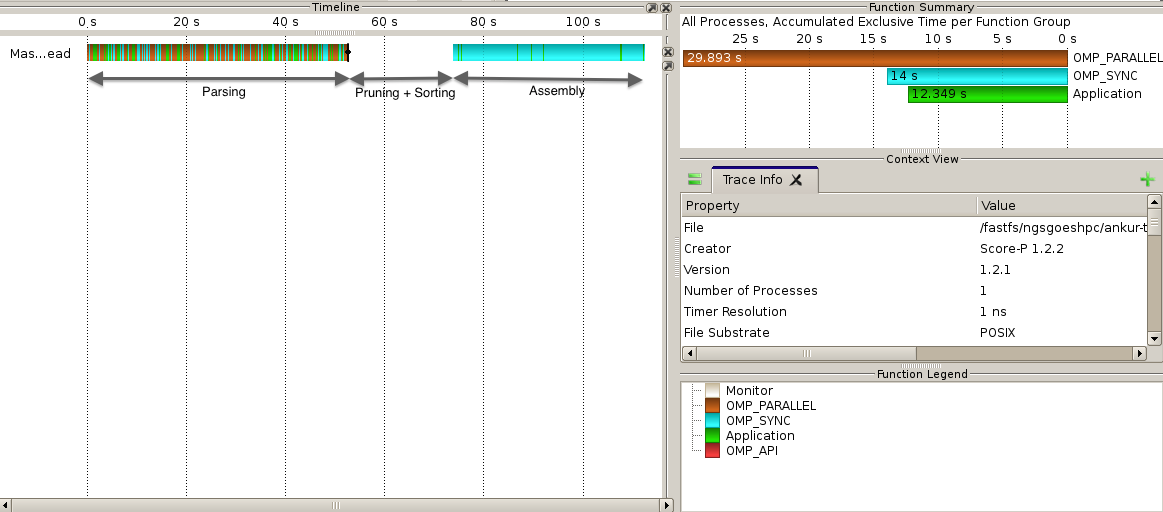
\includegraphics[scale=0.35]{trace-original}
\caption{Trace - Original version of Inchworm, 4M Dataset}
\label{trace-original}
\end{figure}
\section{Analysis of Inchworm}
The thorough analysis requires a deep knowledge of algorithms and techniques implemented in Inchworm. The modular structure uncovered several performance bottlenecks that can be optimized in order to achieve a better performance in terms of results and speed. Trace of the original implementation of Inchworm as shown in figure ~\ref{trace-original}, depicts that all phases of Inchworm are executed by the master thread which means that Inchworm is a pure serial implementation.
\paragraph{}
As shown in figure ~\ref{trace-original}, Inchworm spends around 41\% time in the parsing phase, 20\% time in pruning, 4\% time in sorting and remaining 35\% time in the assembly phase. Since all phases as represented in figure ~\ref{trace-original} are serial, we can obtain a significance speedup without compromising with the quality of the results obtained from Inchworm.
\subsection{Description of algorithms and bottlenecks}
\paragraph{Parsing} 
Inchworm uses large FASTA file generated by Jellyfish as input to generate linear transcripts. It is the only phase of Inchworm that reads data from disk and then extracts the k-mer information from this data to create a k-mer catalog. Since the FASTA file is read only once, parallel random access to this file brings down the performance of application to a great extent as shown in figure ~\ref{disk}. As suggested by \cite{Jacobs}, using multi-threaded pointer to a file that randomly moves across the file to access the information stored on the disk introduces huge overhead. This overhead increases with the size of the file and the number of parallel accesses made to this file. Since the size of FASTA file is usually few Giga-Bytes (~10G), reading the file in a serial manner can prove to be beneficial. But, since the data that is retrieved from the FASTA file needs to be parsed in order to obtain the k-mer information, parallel process of this data using multiple threads can boost the phase by countering the overhead introduced by random read from disk. 
\begin{figure}[h]
\center
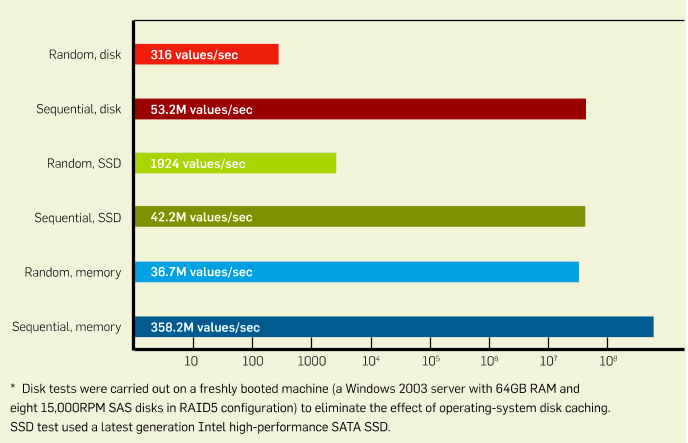
\includegraphics[scale=0.35]{disk}
\caption{Disk Performance: Random v/s Serial Read}
\floatfoot{Source: \cite{Jacobs}}
\label{disk}
\end{figure}
\paragraph{}
Since loading of data from disk takes a very small amount of time when loading large chunk of data at a time (not when reading single k-mer at a time), using fast file systems like RAMDISK and Solid State Disk have a very limited effect on the performance of Inchworm. So for efficient and fast parsing of FASTA file, we have to optimize the parsing of in-memory data. So, rather than parsing the k-mer one by one from the file, we can load the entire data into memory and then can parse the k-mer information by dividing the data among multiple threads.
\paragraph{}
The other problem with this phase of Inchworm is the k-mer catalog which is a hash table storing the key-value pair of k-mer information. The data that is parsed is inserted into this catalog. If we use multiple threads to parse the information, inserting the k-mer pair into this catalog can introduce a lot of overhead as this can only be done inside a critical section. So for each parsed k-mer,  thread waits until other thread finishes inserting the parsed k-mer into hash table. 
\paragraph{Pruning} Removing erroneous k-mers from the catalog is performed sequentially.  Let us consider a 4-mer ATTG with an abundance count of X. The k-mer is removed from the catalog if the abundance count X is less than a specified threshold. Other technique of pruning k-mers evaluates entropy using equation 1, and if the entropy is less than a specified amount, it is removed to prohibit its use in the k-mer extension. The last method extends the k-mer ATTG one step, the extension set includes 4-mers {(TTGA, 323), (TTGC, 132), (TTGT, 0), (TTGG, 987)}. Then using equation ~\ref{eq2} on page ~\pageref{eq2}, ratio of its dominance is evaluated. If this ratio is less than the specified threshold (min\_ratio\_non\_error), the k-mer is removed from the catalog.
\paragraph{}Considering an example, suppose we have a k-mer k that can be extended using k-mers {$k_{1}$,$k_{2}$ and $k_{3}$} and k-mer $k_{2}$ among these extension can be extended using k-mers {$k_{4}$ and $k_{5}$}. If done sequentially, Inchworm removes k-mer $k_{2}$ when it checks for the complexity of k-mer k. So, Inchworm no longer tests k-mer $k_{2}$ for less complex extensions. On the other hand, if we perform this stage of pruning in parallel distributing the work among several threads, if two separate threads perform check for k-mer k \& $k_{2}$, the extension on k-mer $k_{2}$ is also verified for complexity which may end up removing some extra k-mers from catalog. As the number of threads doing pruning increases, the chance of removing the extension k-mer for an already removed k-mer increases which has a significant effect on the final results of Inchworm. So, the amount of k-mers that are pruned when done in parallel depends on the database as well as number of threads that are assigned for pruning . For the  \emph{Drosophila melanogaster} dataset, the parallel implementation ended up removing 5\% more k-mers which slightly deviated the results obtained by Inchworm. This algorithm prohibits parallel implementation of pruning into Inchworm.
\paragraph{Assembly}
This last and the most important phase of Inchworm assembles together the processed k-mer catalog in order to obtain a set of larger linear transcripts. In the current implementation, Inchworm selects the most abundant unused k-mer from the k-mer catalog. It then assembles the k-mer in the forward direction using the k-1 overlapping coverage. After completing the forward extension, it similarly extends the k-mer in the reverse direction. The k-mers that are used in the forward direction are no longer used in the reverse direction by maintaining a set of visited k-mers which is passed to the reverse assembly to make sure no k-mers which are already visited are used. The decision of computing forward assembly first is arbitrary which may result in the change of final results.
\begin{figure}[h]
\center
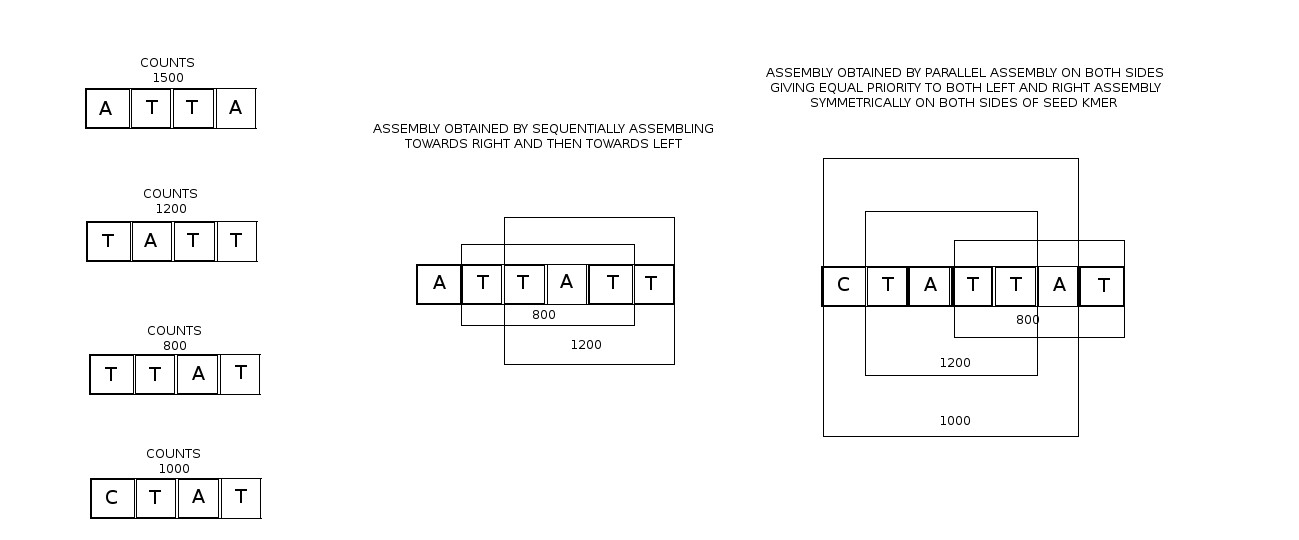
\includegraphics[scale=0.5]{assemble}
\caption{Assembler: Ambiguity in assembly phase}
\label{ambiguity}
\end{figure}
\paragraph{Significance of assembly direction}
Considering the example shown in figure ~\ref{ambiguity}, the assembler selects 4-mer ATTA as a seed k-mer. Using the current implemented algorithm, the assembler extends the seed first in the forward direction and the in the reverse direction. This extension as shown yields the contig ATTATT of length 6 and total abundance count of 2000. But, if we assemble it in the reverse order giving priority to reverse extension, or we allow the same k-mer to be used on both sides for extension in different contigs, and then choose the best extension, we get contig CTATTAT with length 7 and total abundance count of 3000. Since contigs generated by the two approaches are different in length as well as complexity, the direction of assembly does play a crucial role in the assembly procedure. The occurrence of k-mer on either side is determined by two different k-mers and the extensions in these two directions are independent which makes the use of same k-mer on either side symmetrical independent.
\begin{figure}[h]
\center
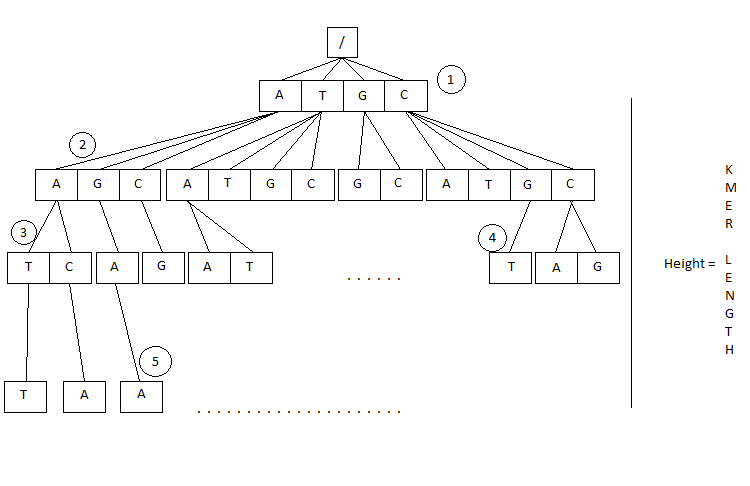
\includegraphics[scale=0.7]{multi-thread}
\caption{Multithreaded memory optimized k-mer catalog}
\label{trie}
\end{figure}
\subsection{Optimization techniques}
\paragraph{Parsing}
I present two techniques to resolve this problem which can be implemented to achieve a significant boost in the parsing phase. First is to use a lock-less hashing such as Hopscotch Hashing as introduced by \cite{hopscotch} or a lockless lookup hash table ~~\cite{tock}. A simple implementation libhash of lock free hash table is available at \cite{lockfree} under open source distribution.
\paragraph{}
The other method is to use a partial locked trie. It can also provide a high degree of parallelism for inserting k-mers into catalog. figure ~\ref{trie} shows how k-mers can be stored in a trie. The first node is a root that marks the beginning of the catalog. To insert a k-mer into this catalog, the thread traces the sequence in the catalog to use the already built nodes until as long as possible. 
\paragraph{}
From figure ~\ref{trie}, suppose we have a catalog of 4-mers, which already has a 4-mer AATT stored in it which means we already have a node / -> A -> A -> T -> T. So for inserting a 4-mer AACA, the catalog is traced until node 2. After this node, the thread needs to create nodes on its own. So it locks node 2, to create a new node with nucleotide C under node 2. It then takes lock over this newly made node, releases the lock from node 2 and creates a node C. This allows other threads to create nodes in parallel therefore allows a large degree of parallelism. As the catalog grows, the amount of overlapping between the k-mer and the already created catalog also increases to a great extent, which in return reduces the probability that two different threads are waiting to get a lock on the same node. The leaf node of this trie holds the k-mer abundance which can be looked up simply by traveling through the catalog trie.
\paragraph{}
This provides a constant time lookup O(k) and constant time insertion O(k), where k is the constant k-mer length. This technique uses high degree of overlapping nodes which reduces the memory consumption to a great extent. So parsing the serially fetched data in parallel using multiple threads and creating trie catalog can greatly boost the performance and reduce the memory consumption to a great extent.
\paragraph{Pruning}
Considering all the three methods of pruning, the first two methods are purely independent as whether a k-mer will be removed or not purely depends on its own dominance and not on other k-mer like the last technique. This implies we can prune the catalog in parallel. These phases can also be integrated in the parsing phase of Inchworm. This will compromise the modular structure of Inchworm distributing the pruning among the two initial stages of Inchworm.
\paragraph{Assembly}
Based on the bottlenecks described, I have designed and implemented a master-slave approach for assembling the k-mers. This technique distributes the process of assembling the k-mers among several workers. The master on the other hand utilizes the precomputations generated by these workers to compute the final contigs. Further section discusses the implementation of these optimization and the effect on these optimization techniques on the overall performance on Inchworm.
%%%%%%%%%%%%%%%%%%%%%%%%%%%%
\newpage
\chapter{Performance Optimization}
Based on the analysis of different phases of Inchworm, many optimization techniques were deployed and tested to achieve a better performance. The following section discusses the optimization techniques used to tune the present implementation of Inchworm, the impact of optimization on the output of Inchworm and the comparison of tuned implementation to the original version. 
\begin{figure}[h]
\center
\includegraphics[scale=0.45]{Inchworm_dfd}
\caption{Dataflow: Optimized Inchworm}
\label{dfd}
\end{figure}
\section{Overview of Optimized Inchworm}
The basic target throughout the optimization procedure of Inchworm was to keep the results of the application as intact as possible. Though some of the optimization alter the results, I have verified that my approach can be tuned in order to obtain the exact similar results of Inchworm. Based on the concepts of distributing the application and data among several threads for parallel processing, defined an overall structure of the parallel Inchworm. Figure ~\ref{dfd} on page \pageref{dfd} shows the exact data-flow in the parallel implementation of Inchworm and explains how each of the phases use the data in order to evaluate final linear transcripts. 
\paragraph{}
The data of the FASTA file generated by \emph{Jellyfish} is mapped in various chunks to memory. This file is then parsed by individual threads to obtain the k-mer information that in stored in a shared k-mer catalog implemented as a hash table. This table is then used to create a list of seed k-mers that is sorted in the descending order of k-mer abundance. The main motive of doing this step is to defer searching for the next most abundant k-mer in the catalog. Once the sorted list of seeds is generated, it is equally distributed among the slaves to generate precomputed extensions. These precomputations are then used by the master thread to create full length linear transcripts. Further thesis discusses the phase wise optimizations implemented and comparison with the original implementation.
\section{Parsing}
As discussed, we tradeoff between the overhead due to parallel random read from the disk and parallel parsing of k-mer information from in-memory data. Various techniques were tested to achieve better performance. Reading k-mer data efficiently into memory is a tedious task. The best technique to load the data of a large file in memory is to use memory mapping. 
As per information on page \cite{mmap}, "Very large blocks (much larger than a page) are allocated with mmap (anonymous or via /dev/zero) by this implementation. This has the great advantage that these chunks are returned to the system immediately when they are freed. Therefore, it cannot happen that a large chunk becomes "locked" in between smaller ones and even after calling free wastes memory. The size threshold for mmap to be used can be adjusted with mallopt. The use of mmap can also be disabled completely". This technique maps the content of a file to the memory and allows us to access the content of the file as if it is loaded into memory. When queried for the data, the operating takes care of the I/O and loads sufficient amount of data into the memory. It loads enough data (more than what is actually queried) into the memory considering that the data will be accessed sequentially. The amount of data that is loaded into memory depends totally on the amount of free memory and the page size. The best part of using this technique is that we can divide the content of file into several chunks in order to process the loaded data in parallel.
\begin{figure}[h]
\center
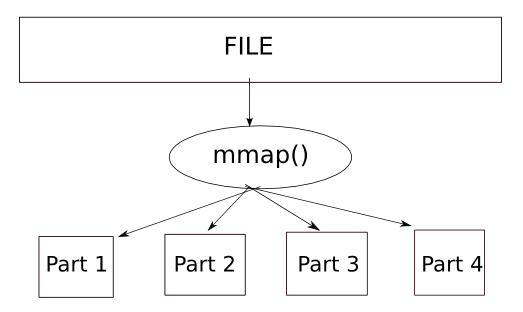
\includegraphics[scale=0.50]{mmapi}
\caption{Memory map}
\label{mmapid}
\end{figure}
\paragraph{}As shown in figure \ref{mmapid}, the gnu mmap() function offers a simple method to map a section of a file into memory. It specifies the offset and the length of data that has to be mapped to the memory. We can mount data of any length using this technique but offset used in this function can only be an integral multiple of page size which can be obtained dynamically using get\_page\_size(). Once mapped, it returns a pointer of void data-type which can then be cast into char\* to be used to fetch the k-mer information. This techniques loads whole FASTA file into memory in chunks and returns the pointer to corresponding chunk. These pointers can then be used to locate and process data which can now be done in parallel without compromising the speedup due to random disk read. 
\paragraph{} The parallel implementation completely alters how the FASTA file is read and parsed to obtain the k-mer information i.e. k-mer sequence and the abundance count. To generate the k-mer catalog, I used a driver function populate\_kmers\_using\_mmap() in the IRKE class file. This function helps Inchworm to memory map the file and parse the data of each of the memory mapped partition. It first maps the file to the memory using the FileMap class to map the file to the memory. This class divides the file into specified number of equal parts. It uses a byte\_offset while dividing the file to make sure it never cuts a k-mer information in between. So, if $i^{th}$ part starts at byte k of the file, the $i-1^{th}$ partition ends at k+\emph{byte\_offset} byte. Once all the partitions are mapped to memory, these partitions are parsed using the IOProcessor class which parses its share of memory mapped file and creates a local buffer of k-mer information. When one of the thread completes parsing its data, it takes a lock over global k-mer hash table and copies all its k-mer information. Once it is done, it releases the lock over the hash table so that other threads can write to it. 
\begin{figure}[h]
\center
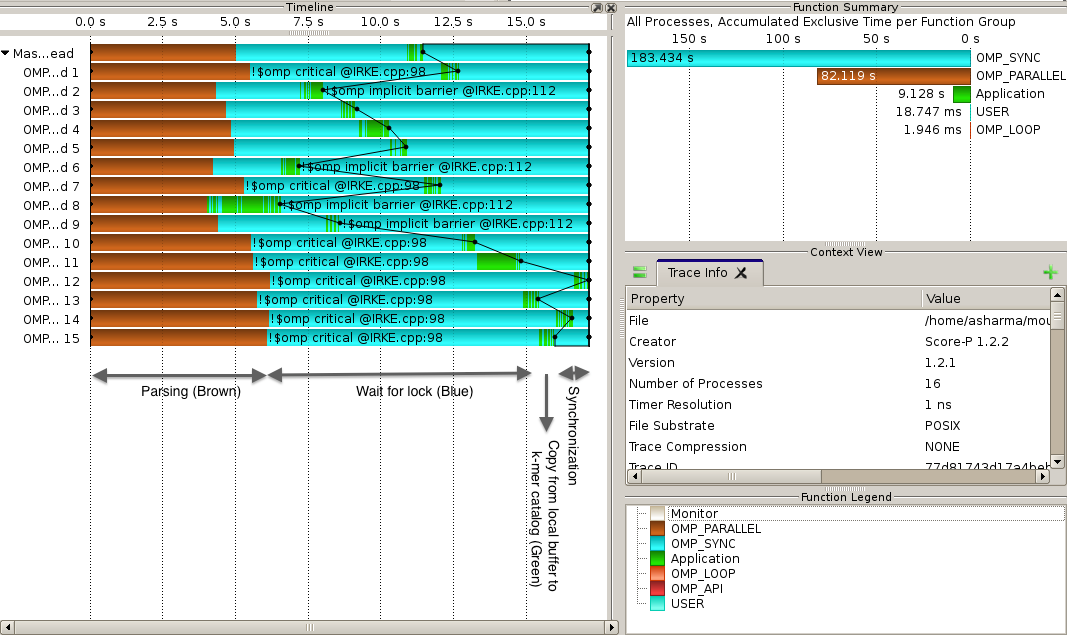
\includegraphics[scale=0.32]{Parse_trace}
\caption{Trace: Parallel Parsing Phase, Dataset: 4M}
\label{trace-parsing}
\end{figure}
\paragraph{}
As shown in figure ~\ref{trace-parsing}, the initial stage represented by brown color indicates the parsing phase where each thread parses its share of memory mapped data and creates a local buffer. Once the thread is finished parsing it waits to take a lock over the shared hash table which is shown in blue color. Once thread gets a lock, it copies the data from the local buffer to the shared data structure represented by the green color. Once it completes, it releases the lock over the hash table and waits until all the treads are done. The black line resembles the control flow and synchronization between the treads. 
\begin{figure}[h]
\center
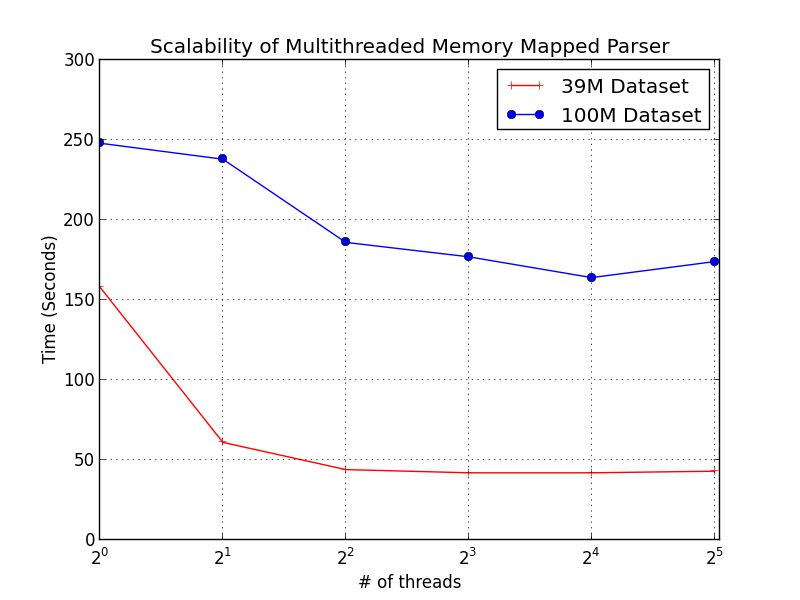
\includegraphics[scale=0.4]{scale_parse}
\caption{Scalability: Memory Mapped Parser}
\label{scale-parser}
\end{figure}
\begin{figure}
\center
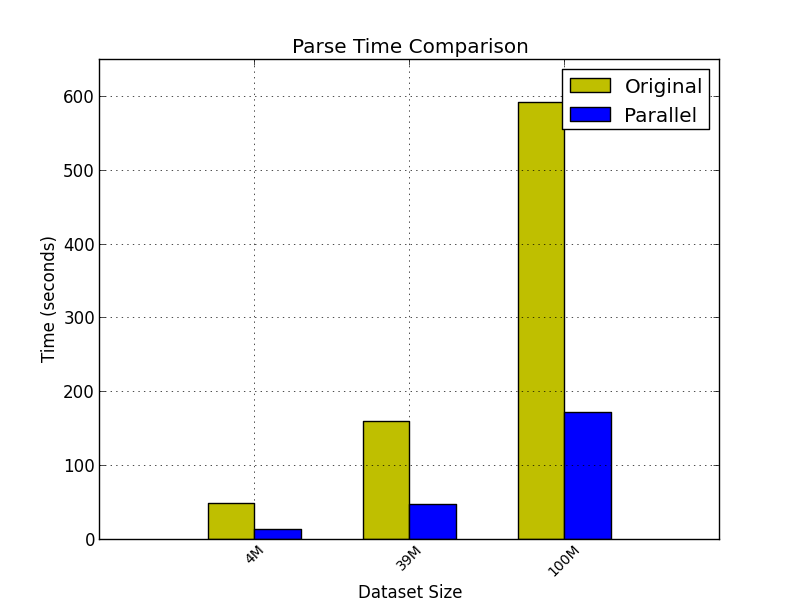
\includegraphics[scale=0.4]{Parse_compare}
\caption{Parsing Comparison: Original v/s Parallel : 16 threads}
\label{compare-parser}
\end{figure}
\paragraph{}
Handing over the disk i/o to the operating system efficiently copies data to the memory which is parsed in smaller chunks by different threads. The concept of distributing this phase among several OpenMP threads greatly enhance the performance of this phase. As shown in figure ~\ref{scale-parser} on page \pageref{scale-parser}, this technique offers scalability until 16 threads. As the number of threads and partitions grow, the amount of data that is parsed by each thread decreases. So the threads finish off very quickly with their parsing. But, due to large number of threads waiting to get a lock over the shared hash table, the overhead increases which brings down the performance of the application. But even though the phase scales to a limited extent, it offers a great performance boost to the application offering a great speedup with a factor of 4. The plot of comparison between the original parsing implementation and the memory mapped parsing is shown in figure ~\ref{compare-parser} on page \pageref{compare-parser}. It clearly shows that as the data-set size grows, the memory mapped parser scales better and provides an efficient way to create a k-mer catalog from the Jellyfish output.
\begin{figure}[h]
\center
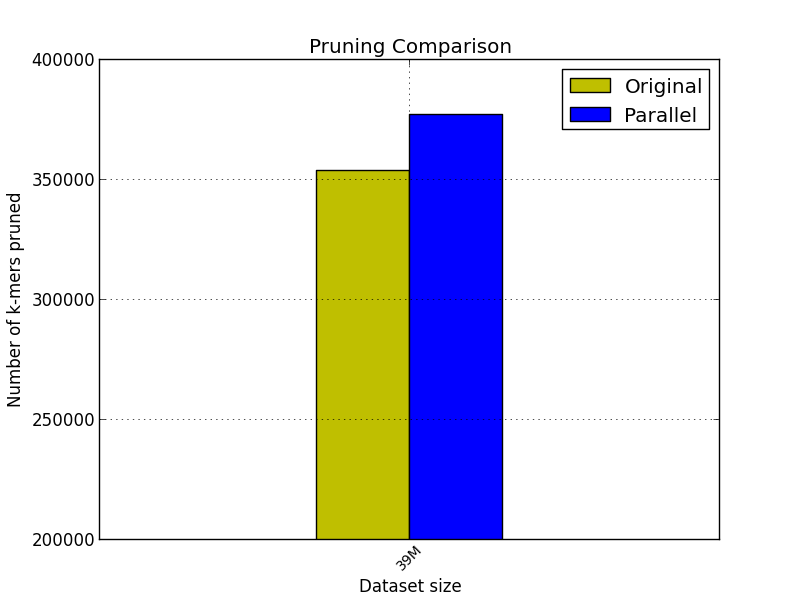
\includegraphics[scale=0.4]{pruning_compare}
\caption{Pruning: Number of k-mers pruned}
\label{compare-pruningnum}
\end{figure}
\section{Pruning}
In the original implementation, pruning phase accounts to almost 20\% of the total run time of Inchworm. As per the analysis of the pruning phase of Inchworm, this phase clearly effects the Inchworm output. Removing the error containing k-mers is pure serial implementation which can surely be transformed into parallel efficient pruning. The parallel implementation of this phase removes approximately 5-10\% more k-mers than the serial implementation. The reason to this issue is clearly explained in performance analysis section. 
\paragraph{}
As shown in figure ~\ref{compare-pruningnum}, the parallel implementation of this phase removes around 6\% more k-mers when tested on a 39M data-set. Since the probability of overlapping of k-mers considering the same k-mer is a possible extension of more than one base k-mers is very low, so removing the extensions of already pruned k-mer has a negligible effect on the overall performance of Inchworm. Although we get slight variation in the result, this phase can also be tuned in order to obtain exact same result as the original implementation. The first two techniques of pruning on the basis of counts and entropy are independent of other k-mers. So these two methods can be executed in parallel using multiple threads to obtain a better scalability. As shown in figure ~\ref{compare-pruning}, the parallel version of this phase is almost 3X faster than the current implementation but it alters few of the linear transcripts generated by Inchworm.
\begin{figure}[h]
\center
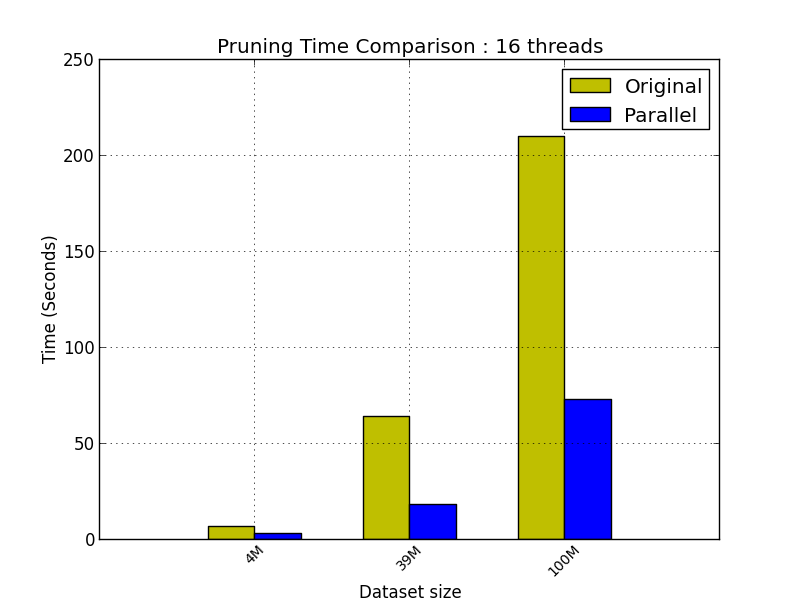
\includegraphics[scale=0.5]{compare-pruning}
\caption{Pruning: Runtime Comparison}
\label{compare-pruning}
\end{figure}
\section{Assembly}
Since the conventional greedy way of assembling the sequence randomly prefers forward assembly over reverse assembly, the approach just does not seem to be totally symmetrical. If we choose to assemble in reverse order giving preference to the reverse assembly over the forward assembly, the results are significantly altered. This change in results may or may not have a serious impact on the biological relevance of the results obtained by running whole Trinity package. But this symmetrical behavior can be retained by allowing the occurrence of k-mer on both sides of an extension. Since the k-mers are removed from the catalog once they have been used in the extension on either direction, the same k-mer can no longer be used on the other side. As illustrated in figure ~\ref{ambiguity} on page \pageref{ambiguity}, the position of the k-mer on either side of the assembly is guided entirely by different k-mers, and the following extension of a k-mer on either direction is entirely different unless the k-mer sequence is a palindrome, the same k-mer when used in both direction may lead to better results. As per the test run on the Drosophila melanogaster data-set, the approach resulted in more number of contigs with better length.
\paragraph{} This approach also separates both forward and reverse assembly as two independent steps which allows us to run each of them in parallel. In further section, I have discussed a master-slave approach of assembling contig that can boost the performance of the application to some extent. Figure  ~\ref{ambiguity} on page \pageref{ambiguity}, clearly illustrates a scenario where a k-mer has a better position on the other side of the contig but since the k-mer is already used in forward extension, it is removed from the catalog. This ambiguity in the approach of assembly is taken into account when we assemble both the sides of contig independently.
\subsection{Master-Slave Approach}
I have used a standard master slave approach for doing the assembling in parallel. The master thread creates some workers for forward and reverse assembly and distributes the seed list among them equally. The workers then select a seed from their share of seed list, assemble in one of the directions and store this half evaluated contig in a hash table which is shared among the workers and the master. The master now can directly look up this hash table for pre-evaluated results and use them for assembling. Once the master gets a pre-evaluated result, it verifies the assembly by checking that the k-mers used in the extension are not already removed from the catalog. If the contig somehow fails to satisfy any criteria, the master itself does the assembly which is always valid in any case. Once the assembling is complete in both directions, the master marks the k-mers that were used in the assembly as used and they will no longer be used for the assembly. The workers do not mark the k-mers, but once they are marked by the master, the workers do not use these k-mers for extension.
\subsection{Source Code Changes}
The parallel implementation of this last stage of Inchworm slightly alters the assembly algorithm as explained in the performance analysis part of this documentation. Doing forward and reverse assembly in parallel allows fully symmetrical merging of k-mers. 
\paragraph{}
To ensure that a k-mer is used only once in each direction, I have used two bits in the data structure that holds the k-mer abundance value. Since the maximum value that can be stored after reserving 2-bits is $2^{30}-1$, we have enough space to hold the abundance count for the largest possible data-sets. The left bit of these two bits is used for marking that the k-mer is already used for the reverse extension. Similarly the right bit when set signifies the k-mer is already used for the extension in the forward direction.
\begin{figure}[h]
\center
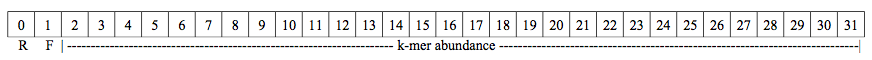
\includegraphics[scale=0.5]{bit}
\caption{Bit manipulation in k-mer abundance data structure}
\label{bit}
\end{figure}
\paragraph{}
In figure ~\ref{bit}, R denotes the flag which is set when the k-mer is used in the reverse assembly and F denoted the flag that is set when it is used in the forward assembly. This bit manipulation technique is much faster than deleting an entry from the hash table and requires only a set of AND and OR operations. When selecting a k-mer as seed, the parallel assembly verifies that neither of these flags are already set. Which means that the k-mer is not yet used in the forward or reverse assembly in previous assembly process. So in order to mark the k-mers, it no longer needs to remove the k-mer from the catalog or set its count to zero, but it just sets the appropriate flag which prohibits its further usage in the assembly in the same direction.
\paragraph{}
The parallel version of this phase gets a sorted list of k-mers which is then used as a seed list by the master as well as the workers. The whole Inchworm phase consists of a master and few slaves or workers. The seed list is equally divided between all the workers. Initially same worker was responsible for calculating the forward as well as the reverse extension of a k-mer. But since the OpenMP thread pool uses a fork-join concept thats blocks the thread until both of the forward and reverse assembly is finished, it introduced a lot of overhead. So, the work of forward as well as the reverse assembly are now distributed among different threads. So, if it creates 10 workers, 5 work to evaluate forward assembly of the equally distributed seed list and the other 5 evaluate the reverse extension. This reduced a lot of unnecessary overhead due to the blocking of threads. The workers were also tuned to reject the k-mers that are previously used to avoid unnecessary extension by checking whether it has a valid entry in the hash table. If the k-mer flag has been set in the hash table, the workers reject it as a valid seed k-mer. The workers write the evaluated extensions to the shared hash table which is then used by the master to obtain the pre computed extensions. The parallel version uses two hash tables to store the precomputed extensions, one storing the forward extensions of the k-mer and the other storing the reverse extension.
\begin{figure}[h]
\center
\includegraphics[scale=0.27]{trace_parallel_Inchworm}
\caption{Trace: Parallel Inchworm, Dataset: 4M}
\label{assemble-trace}
\end{figure}
\paragraph{}
The master selects a seed k-mer, checks the hash tables for precomputed extensions, verifies that no k-mers used in these extensions are already used and joins them together to obtain the linear transcript. If the master finds out that either of the precomputed extension is faulty, it recomputes that extension which is surely genuine. Master is the only thread that marks the k-mers as used and no other thread have access to such a facility. This enables us to counter any race condition that may arise due to multiple markings on the same k-mer. Although this assembly technique alters the result of Inchworm, we can tune the master to obtain the full serial version of assembly producing exactly similar result as the original implementation. Serializing the assembly in the master and passing the visitor set that holds the k-mers that are used in the forward extension to the reverse assembly are the only two steps that can tune the parallel version to obtain similar behavior as the original implementation.
\subsection{Benefits}
The parallel implementation of assembly phase provides a slight speedup of around 20\% restricting the assembly time (39M Data-set) of 104 seconds of original implementation to just 82 seconds. As shown in figure ~\ref{assemble-trace}, 4 workers compute the extensions in parallel which is used by the master thread for assembly. Based on the tiny data-set (4M kmers), around 90\% of the extensions computed by master uses the pre computed assembly stored in the hash table. Out of these only 5\% of the extensions were found to be faulty and was recomputed by the master.  For a 39M dataset, for about 1\% extensions evaluated by master, the precomputed right and left extensions were never actually found in the hash table. Where as for 99\% of assembly used the precomputations evaluated by the slaves, only  5\% (forward extension) and 10\%(reverse extension) were found to be invalid and had to be recomputed by the master. 
\paragraph{}
The speedup obtained in the parallel implementation is very limited due to high level of verification procedure performed by the master. The master makes sure that same k-mer is not used more than once in the assembly, this can only be done by checking individually each of the k-mers used in the precomputation. This verification procedure hinders the speedup obtained by precomputing extensions by increasing the workload on the master. The master has to hit the k-mer catalog for each k-mer present in the precomputed extension which is almost the same amount of work that it needs to perform in computing the extension by 
itself.
\begin{figure}[h]
\center
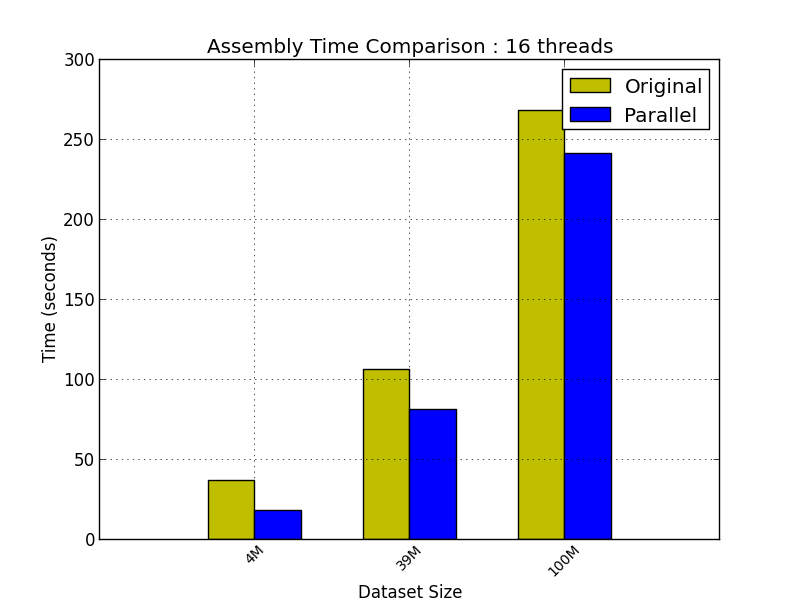
\includegraphics[scale=0.45]{compare-assembly}
\caption{Assembly : Runtime Comparison}
\label{assembly-compare}
\end{figure}
\paragraph{}
As shown in figure ~\ref{assembly-compare}, the master slave approach of assembling k-mers provides a slight speedup. But, the idea of using the k-mers on both sides of seed k-mer relatively ensures a better level of symmetry, produces slighty longer contigs and also higher number of linear transcripts. 
%%%%%%%%%%%%%%%%%%%%%%%%%%%%
\newpage
\newpage
\chapter{Conclusion}
The parallel implementation of Inchworm has significant effect on the performance as well as its results. Even though there is not much speedup in the assembly phase of the application, speedup of parsing and pruning phase deliver a decent speedup to the module.
\section{Results}
Considering the Drosophila melanogaster test dataset containing 39M k-mers, the implementation reported a boost of 2 times in the parallel phase, 3 times in the pruning phase as shown in figure ~\ref{drozo}. The parallel implementation of Inchworm reported 17\% more contigs with a good increment of 28\% in the count of base pairs. The total time of execution of parallel Inchworm with this dataset was 142 seconds compared to 306 seconds of the serial Inchworm implementation. No difference in the maximum and minimum length of contigs were reported in the two implementations. Parallel Inchworm also reports 6\% increase in the N50 length of the reported linear transcripts which shows a significant improve in the quality of transcripts. 
\begin{figure}[h]
\center
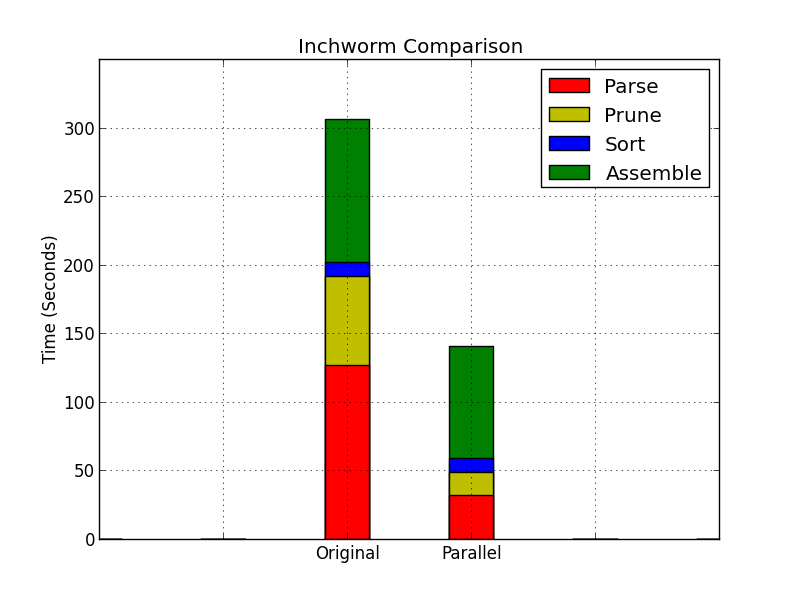
\includegraphics[scale=0.45]{inch_compare}
\caption{Inchworm: Overall comparison with 16 threads, Dataset: Drosophila melanogaster (39M k-mers)}
\label{drozo}
\end{figure}
\begin{figure}[h]
\center
\includegraphics[scale=0.45]{compare-Inchworm-schizo}
\caption{Inchworm: Overall comparison with 32 threads, Dataset: Schizosaccharomyces pombe (240M k-mers)}
\label{schizo}
\end{figure}
\begin{table}
\begin{center}
\begin{tabular}{| c | c | c | c | c | c |}        
\hline            
Dataset Name & \# Contigs & \# Base Pairs & \# Max Length & \# N50 Count & \# Runtime (secs) \\	\hline
39M[1] & 128,426 & 24,051,266 & 11,235 & 609 & 306 \\ \hline
39M[2] & 150,342 & 30,947,748 & 11,235 & 646 & 142 \\ \hline
Schizo[1] & 1,448,757 & 73,681,874 & 17,806 & 49 & 2019 \\ \hline
Schizo[2] & 1,758,751 & 102,085,873 & 17,708 & 51 & 1040 \\
\hline  
\end{tabular}
\end{center}
\caption{Comparison of [1] Original implementation of inchworm and [2] Parallel inchworm}
\end{table}
\paragraph{}
The parallel Inchworm when tested against the Schizosaccharomyces pombe dataset containing 240M k-mers also yielded a significant boost in performance. There was a  21\% increase in the number of reported contigs  with a much significant boost of 35.8\% in the count of base pairs. The N50 length also increased from 49 in the original implementation to 51 in the parallel version. As shown in figure ~\ref{schizo}, parallel implementation took 17 minutes 20 seconds compared to 33 minutes 39 seconds which boosts the application by approximately 2 times incorporating 3 times speedup in the parsing and pruning phase.
\paragraph{}
Parallel implementation does not offer a significant speedup in the assembly phase. But due to high speedup of parsing phase (3X) and pruning phase (3X), which share almost 70\% of the total execution time of Inchworm, the observed speedup of the application is about 2. This thesis also describes a better symmetrical approach of assembly which produces more, larger and better linear transcripts with greater base pair count and N50 length.

\section{Future Work}
Though this thesis introduces a significant speedup to the application, Inchworm can still be tuned to a great extent. The current hash table can be replaced with a lock-free hash table removing the synchronization overhead. Using hopscotch ~\cite{hopscotch} or other hashing technique ~\cite{tock} will boost the memory mapped parser to a great extent. A platform to share the in-memory hash table between jellyfish and Inchworm can also be a great step in performance tuning of Trinity as a whole. So, if the user runs whole Trinity package together, Inchworm knows how to grab the in-memory data of Jellyfish which can avoid the overhead of dumping the k-mer information to a FASTA file and reading it again in Inchworm. 
\end{document}
